%!TEX root = ../bare_jrnl.tex

\section{Evaluation on Synthetic Data}
\label{sec:evasim}

In this section we evaluate POPP and its extensions on synthetic data to demonstrate the properties of these models when estimating the arrival rate $\lambda$ of a Poisson process. With synthetic data, sensor reliability can be controlled, and the true $\lambda$ and the true counts $c_i$ can be known for each sample.

% Here, an evaluation and a comparison of the POPP models to the FOPP model are conducted with two imaginary unreliable sensors and simulated datasets. The switching filter is chosen as a filter for all POPP models for this evaluation. 

In our experiments we initially generate a training set of $n=120$ counts from a Poisson process $P(c \mid \lambda'=3)$ and the corresponding sensed counts $\protect\mathbf{s_1} \ldots \protect\mathbf{s_{120}}$ from two unreliable sensors (i.e. $m=2$ in our evaluation). To capture a range of possible sensor correlations and performance characteristics, the sensed counts for the training set are produced from 12 different sensor configurations. The true and sensed counts are then used to build (joint where appropriate) sensor models for the POPP extensions described above. We then generate a new set of $n=144$ true counts and the corresponding sensed counts for each of the 12 sensor configurations. These sensed counts are used as input in a filtering process to estimate the posterior of lambda according to each of the four models defined above (POPP, POPP-Beta, C-POPP, and POPP-Dirichlet), plus FOPP.
% 
We chose the training set size $n=120$ such that there is insufficient data to build an accurate sensor model. This allows the POPP-Dirichlet and the POPP-Beta models to compensate with loose Dirichlet and beta densities. 

The 12 sensor configurations mentioned previously represent 12 different experimental conditions under which we can test our proposed models. In six of the configurations we vary the true joint positive rates (true $P^+$) of the two sensors whilst fixing their true joint negative rates (true $P^-$). In the other six we fix the true joint positive rates (TJPRs) whilst varying the true joint negative rates (TJNRs). Both cases cover variations where the sensors are uncorrelated, positively correlated and negatively correlated, and in each case where the overall true (postive or negative) rates are either high (0.9) or low (0.1). The detailed configurations are presented in Table~\ref{tab:eval_sim}. 



\begin{table*}
\begin{center}
 \begin{tabular}{| c | c || c | c | c | c || c | c | c | c|} 
 \hline
     & $e_k$ &  \multicolumn{4}{|c||}{1} &  \multicolumn{4}{c|}{0} \\
 \hline
 & $d_{1,k}, d_{2,k}$  & 0, 0 & 0, 1 & 1, 0 & 1, 1 & 0, 0 & 0, 1 & 1, 0  & 1, 1\\  
 \hline\hline
 \textbf{TJPR} & \textbf{TJNR} &  &  &  &  &  &  &  & \\  
 \hline
 \hline
 low positive correlation & fixed & 0.1 & 0.0 & 0.0 & 0.9 & 1.0 & 0.0 & 0.0 & 0.0\\  
 \hline
 high positive correlation & fixed & 0.9 & 0.0 & 0.0 & 0.1 & 1.0 & 0.0 & 0.0 & 0.0\\  
 \hline
 low negative correlation & fixed & 0.0 & 0.05 & 0.05 & 0.9 & 1.0 & 0.0 & 0.0 & 0.0\\  
 \hline
 high negative correlation & fixed & 0.0 & 0.45 & 0.45 & 0.1 & 1.0 & 0.0 & 0.0 & 0.0\\  
 \hline
 no correlation & fixed & 0.033 & 0.033 & 0.033 & 0.901 & 1.0 & 0.0 & 0.0 & 0.0\\  
 \hline
 no correlation & fixed & 0.3 & 0.3 & 0.3 & 0.1 & 1.0 & 0.0 & 0.0 & 0.0\\  
 \hline
 fixed & low positive correlation  & 0.0 & 0.0 & 0.0 & 1.0 & 0.9 & 0.0 & 0.0 & 0.1\\  
 \hline
 fixed & high positive correlation  & 0.0 & 0.0 & 0.0 & 1.0 & 0.1 & 0.0 & 0.0 & 0.9\\  
 \hline
 fixed & low negative correlation  & 0.0 & 0.0 & 0.0 & 1.0 & 0.9 & 0.05 & 0.05 & 0.0\\  
 \hline
 fixed & high negative correlation  & 0.0 & 0.0 & 0.0 & 1.0 & 0.1 & 0.45 & 0.45 & 0.0\\  
 \hline
 fixed & no correlation  & 0.0 & 0.0 & 0.0 & 1.0 & 0.9 & 0.033 & 0.033 & 0.033\\  
 \hline
 fixed & no correlation  & 0.0 & 0.0 & 0.0 & 1.0 & 0.1 & 0.3 & 0.3 & 0.3\\  
 \hline
\end{tabular}
\end{center}
\caption{The sensor configurations for the evaluation on synthetic data.}
\label{tab:eval_sim}
\end{table*}


\begin{figure}[t!]
	\centering
	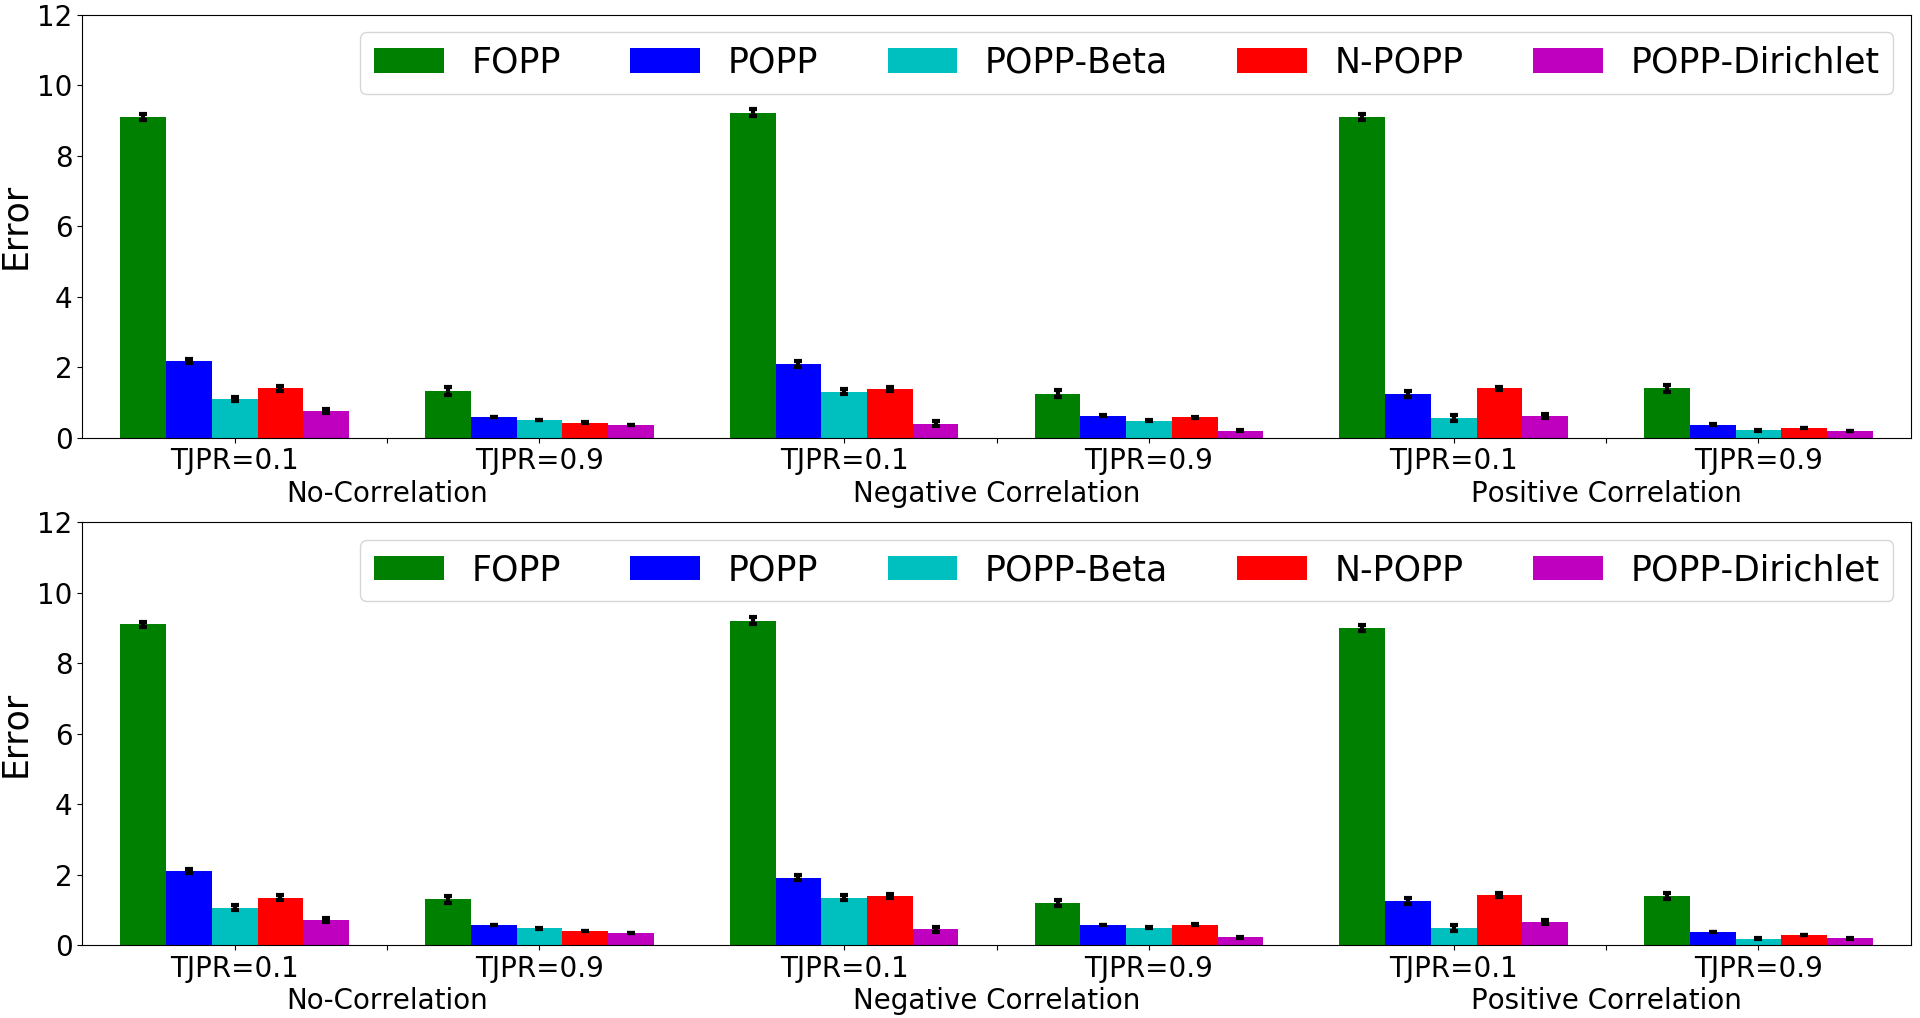
\includegraphics[width=0.5\textwidth]{./figures/tjpr_comparison_120.png}
    \caption{The RMSE of posterior estimates of $\lambda$ for the POPP and its variation models with 120 sample data used to build the (joint) sensor model with variation on $\mathcal{E^+}$. All models are compared to the FOPP model. Each trial consisted of a stream of $\protect\mathbf{s_1} \ldots \protect\mathbf{s_{144}}$ samples to update $P(\lambda \mid \protect\mathbf{s_i})$. Accuracies of MAP estimates are shown in the top panel, accuracies of expectation of the posterior in the bottom panel. Each data point is an average of 30 trials. Standard errors are shown.} 
	\label{fig:tjpr_comparison_120}
\end{figure}

\begin{figure}[t!]
	\centering
	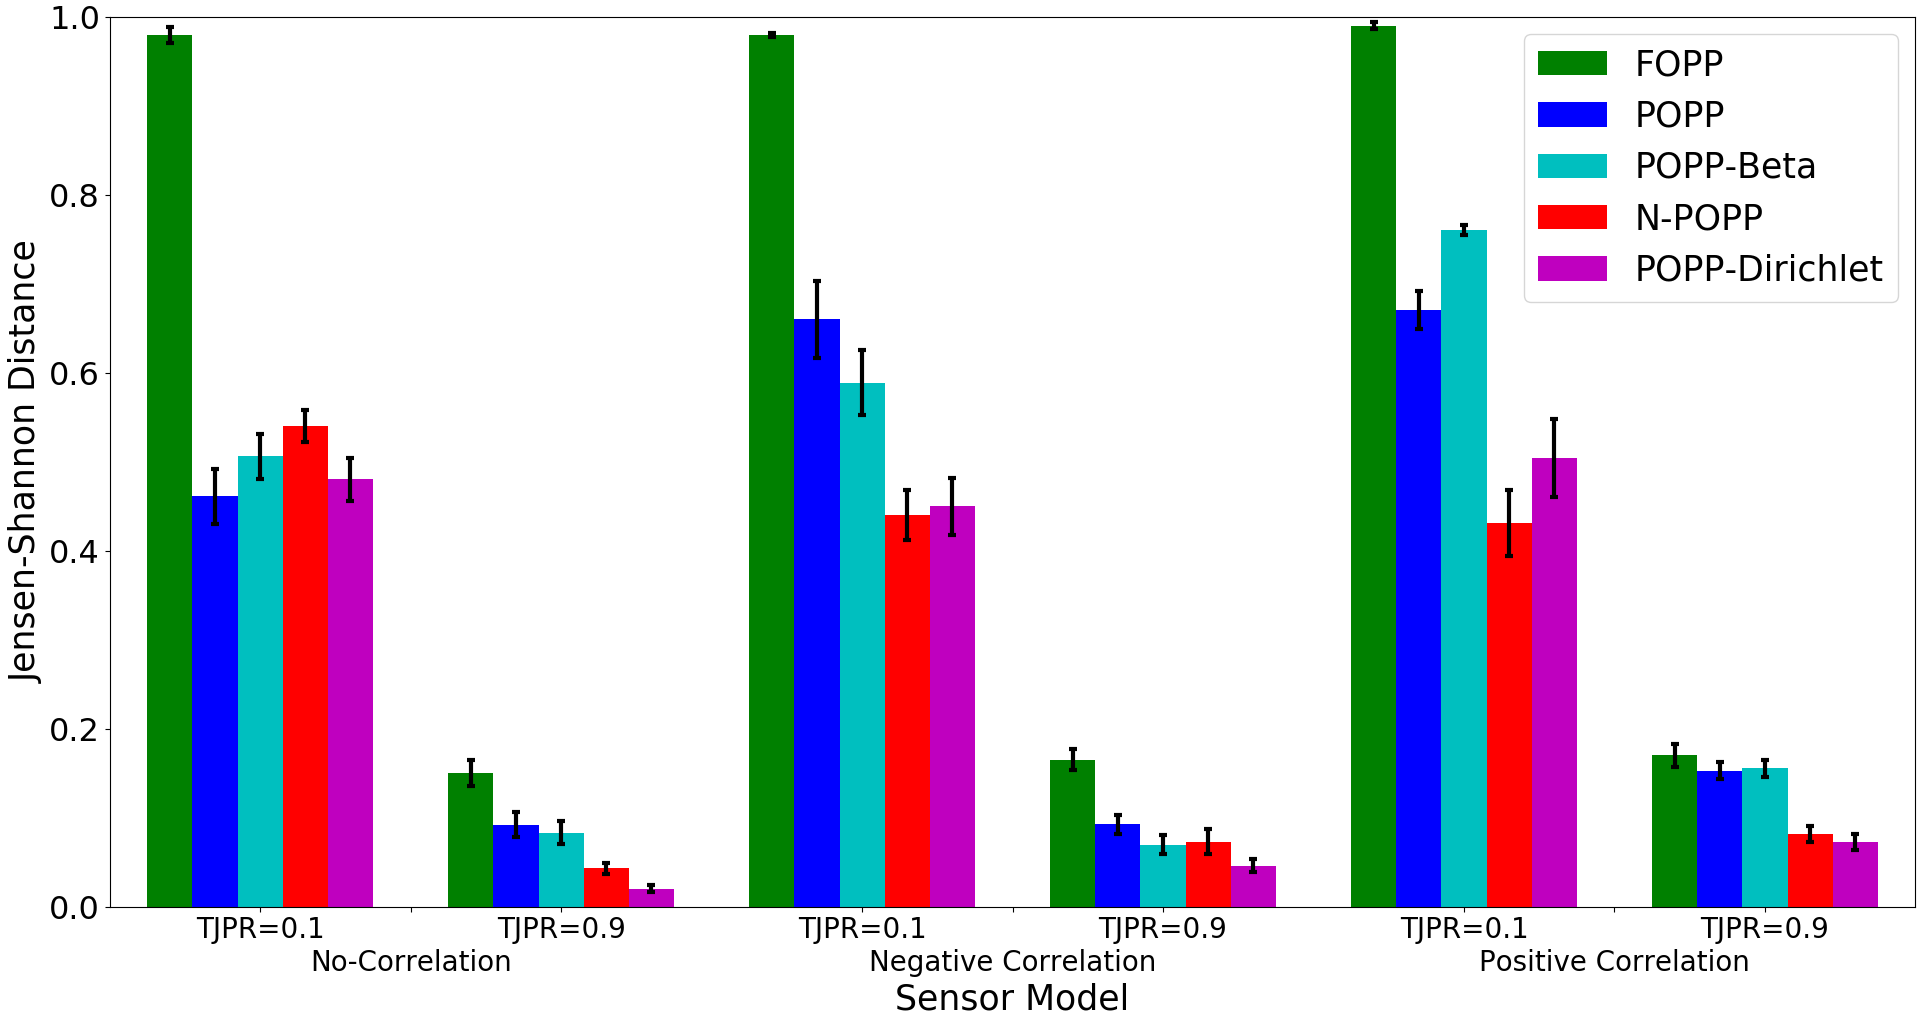
\includegraphics[width=0.5\textwidth]{./figures/tjpr_comparison_120_kl.png}
	\caption{The Jensen-Shannon distance of posterior estimates of $\lambda$ for the POPP and its variation models with 120 sample data used to build the (joint) sensor model with variation on $\mathcal{E^+}$. All models are compared to the FOPP model. Each trial consisted of a stream of $\protect\mathbf{s_1} \ldots \protect\mathbf{s_{144}}$ samples to update $P_G(\lambda \mid \protect\mathbf{s_i})$. Each data point is an average of 30 trials. Standard errors are shown.} 
	\label{fig:tjpr_comparison_120_kl}
\end{figure}

% Different correlations between two sensors were tested: positive correlation, negative correlation, and no correlation. These correlations are aimed to show the benefit of the C-POPP and POPP-Dirichlet models over the POPP and the POPP-Beta models. One should note that under the POPP and POPP-Beta models, sensors are assumed to be uncorrelated. For each correlation type, a further variation to different levels of sensor unreliability was considered. The true joint positive rate $\mathcal{E^+}$ (TJPR) and the true joint negative rate $\mathcal{E^-}$ (TJNR) were set as basis for varying sensor unreliability. For example, having TJPR configured with $P_{jnt}(d_{1k}=1, d_{2k}=1 ; e_k=1) = 0.1, P_{jnt}(d_{1k}=0, d_{2k}=0 ; e_k=1) = 0.9$ means that the true positive rate (TPR) for each sensor $j$ is $\textrm{\textit{tpr}}_j = P_j(d_k = 1; e_k=1) = 0.1$.

% First, two variations were made to the true joint positive rate $\mathcal{E^+}$ (TJPR), while fixing the true joint negative rate $\mathcal{E^-}$ (TJNR) on each type of correlation. This includes:
% \begin{itemize}
%     \item $P_{jnt}(d_{1k}=1, d_{2k}=1 ; e_k=1) = 0.1, P_{jnt}(d_{1k}=0, d_{2k}=0 ; e_k=1) = 0.9$ ($\mathcal{E^+}$ with low positive correlation);
%     \item $P_{jnt}(d_{1k}=1, d_{2k}=1 ; e_k=1) = 0.9, P_{jnt}(d_{1k}=0, d_{2k}=0 ; e_k=1) = 0.1$ ($\mathcal{E^+}$ with high positive correlation);
%     \item $P_{jnt}(d_{1k}=1, d_{2k}=0 ; e_k=1) = 0.05, P_{jnt}(d_{1k}=0, d_{2k}=1 ; e_k=1) = 0.05, P_{jnt}(d_{1k}=0, d_{2k}=0 ; e_k=1) = 0.9$ ($\mathcal{E^+}$ with low negative correlation);
%     \item $P_{jnt}(d_{1k}=1, d_{2k}=0 ; e_k=1) = 0.45, P_{jnt}(d_{1k}=0, d_{2k}=1 ; e_k=1) = 0.45, P_{jnt}(d_{1k}=0, d_{2k}=0 ; e_k=1) = 0.1$ ($\mathcal{E^+}$ with high negative correlation);
%     \item $P_{jnt}(d_{1k}=1, d_{2k}=0 ; e_k=1) = 0.033, P_{jnt}(d_{1k}=0, d_{2k}=1 ; e_k=1) = 0.033, P_{jnt}(d_{1k}=1, d_{2k}=1 ; e_k=1) = 0.033, P_{jnt}(d_{1k}=0, d_{2k}=0 ; e_k=1) = 0.901$ ($\mathcal{E^+}$ with no correlation -- Similar to a sensor model with TPR = 0.066);
%     \item $P_{jnt}(d_{1k}=1, d_{2k}=0 ; e_k=1) = 0.3, P_{jnt}(d_{1k}=0, d_{2k}=1 ; e_k=1) = 0.3, P_{jnt}(d_{1k}=1, d_{2k}=1 ; e_k=1) = 0.3, P_{jnt}(d_{1k}=0, d_{2k}=0 ; e_k=1) = 0.1$ ($\mathcal{E^+}$ with no correlation -- Similar to a sensor model with TPR = 0.6).
% \end{itemize}

% Second, two variations to the true joint negative rate $\mathcal{E^-}$ (TJNR), while fixing the true joint positive rate $\mathcal{E^+}$ (TJPR) on each type of correlation. This includes: 
% \begin{itemize}
% 	\item $P_{jnt}(d_{1k}=1, d_{2k}=1 ; e_k=0) = 0.1, P_{jnt}(d_{1k}=0, d_{2k}=0 ; e_k=0) = 0.9$ ($\mathcal{E^-}$ with low positive correlation);
% 	\item $P_{jnt}(d_{1k}=1, d_{2k}=1 ; e_k=0) = 0.9, P_{jnt}(d_{1k}=0, d_{2k}=0 ; e_k=0) = 0.1$ ($\mathcal{E^-}$ with high positive correlation);
% 	\item $P_{jnt}(d_{1k}=1, d_{2k}=0 ; e_k=0) = 0.05, P_{jnt}(d_{1k}=0, d_{2k}=1 ; e_k=0) = 0.05, P_{jnt}(d_{1k}=0, d_{2k}=0 ; e_k=0) = 0.9$ ($\mathcal{E^-}$ with low negative correlation);
% 	\item $P_{jnt}(d_{1k}=1, d_{2k}=0 ; e_k=0) = 0.45, P_{jnt}(d_{1k}=0, d_{2k}=1 ; e_k=0) = 0.45, P_{jnt}(d_{1k}=0, d_{2k}=0 ; e_k=0) = 0.1$ ($\mathcal{E^-}$ with high negative correlation);
% 	\item $P_{jnt}(d_{1k}=1, d_{2k}=0 ; e_k=0) = 0.033, P_{jnt}(d_{1k}=0, d_{2k}=1 ; e_k=0) = 0.033, P_{jnt}(d_{1k}=1, d_{2k}=1 ; e_k=0) = 0.033, P_{jnt}(d_{1k}=0, d_{2k}=0 ; e_k=1) = 0.901$ ($\mathcal{E^-}$ with no correlation -- Similar to a sensor model with low TNR);
% 	\item $P_{jnt}(d_{1k}=1, d_{2k}=0 ; e_k=0) = 0.3, P_{jnt}(d_{1k}=0, d_{2k}=1 ; e_k=0) = 0.3, P_{jnt}(d_{1k}=1, d_{2k}=1 ; e_k=0) = 0.3, P_{jnt}(d_{1k}=0, d_{2k}=0 ; e_k=1) = 0.1$ ($\mathcal{E^-}$ with no correlation -- Similar to a sensor model with moderate TNR).
% \end{itemize}

The performance of all POPP models was assessed by measuring how accurate each model is in estimating the true $\lambda'$. Two options were used to measure the accuracy: (1) the RMSE of the expectation (mean) and the MAP hypothesis (mode) of each model posterior distribution over $\lambda$ to the true $\lambda'$; and (2)  the Jensen-Shannon distance between the posterior distribution $P(\lambda \mid \mathbf{s_i})$ and the distribution of the true $\lambda'$. 

\begin{figure}[t!]
	\centering
	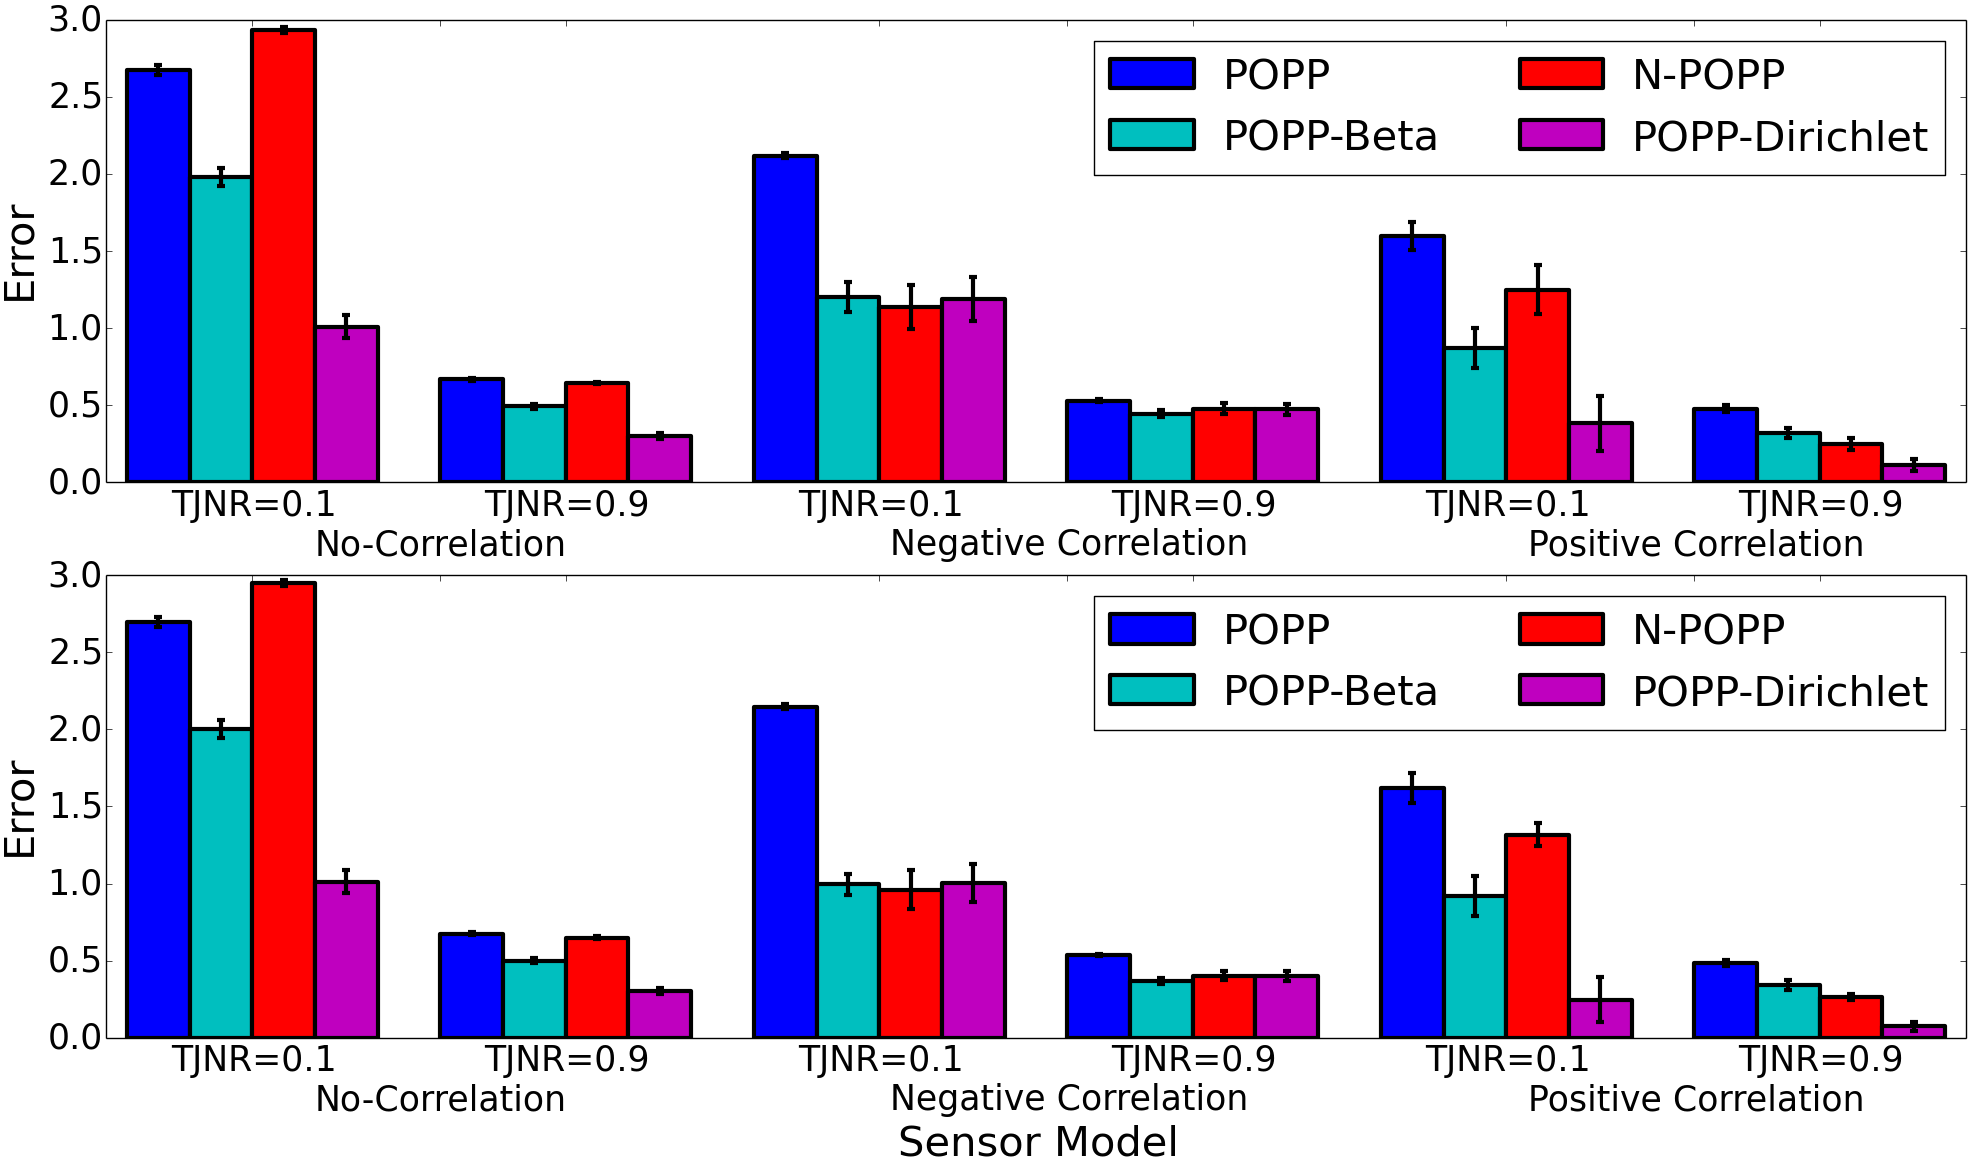
\includegraphics[width=0.5\textwidth]{./figures/tjnr_comparison_120.png}
    \caption{The RMSE of posterior estimates of $\lambda$ for the POPP and its variation models with 120 sample data used to build the (joint) sensor model with variation in $\mathcal{E^-}$. All models are compared to the FOPP model. Each trial consisted of a stream of $\protect\mathbf{s_1} \ldots \protect\mathbf{s_{144}}$ samples to update $P(\lambda \mid \protect\mathbf{s_i})$. Accuracies of MAP estimates are  in the top panel, accuracies of the expectation of the posterior in the bottom panel. Each data point is an average of 30 trials. Standard errors are shown.} 
	\label{fig:tjnr_comparison_120}
\end{figure}

\begin{figure}[t!]
	\centering
	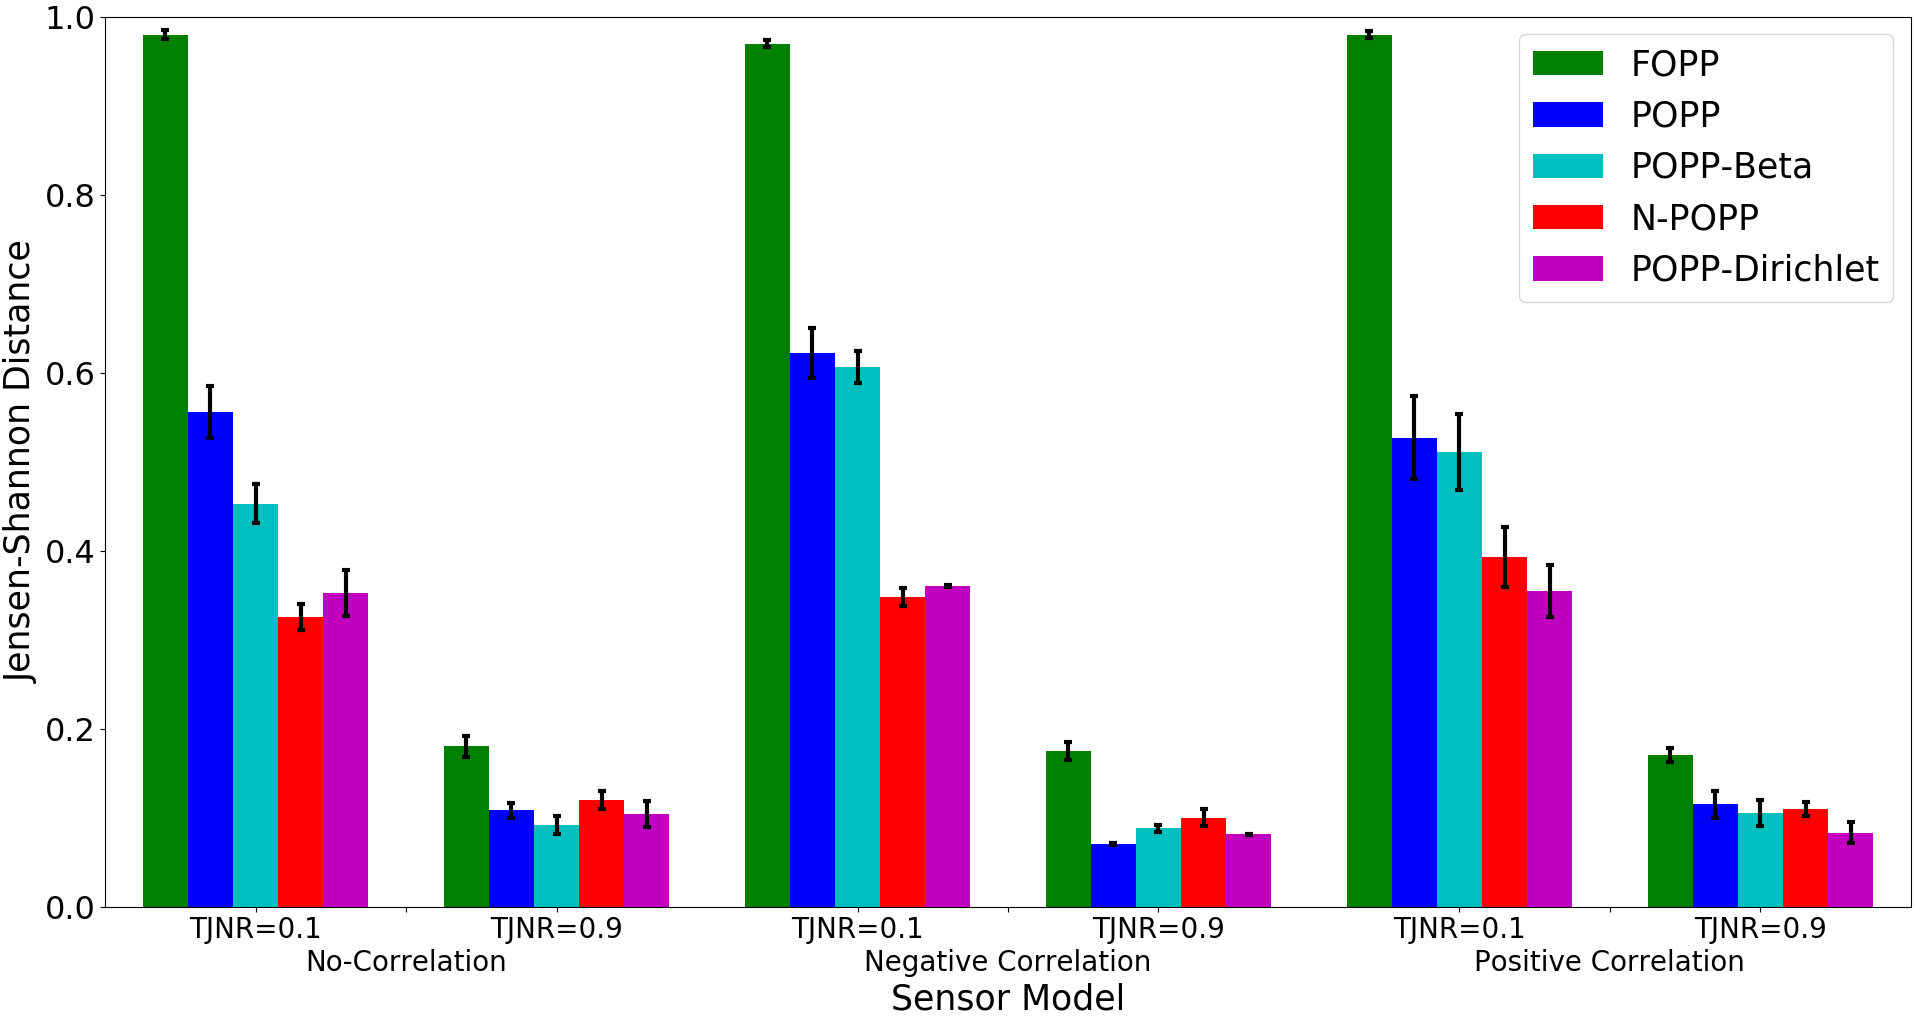
\includegraphics[width=0.5\textwidth]{./figures/tjnr_comparison_120_kl.png}
	\caption{The Jensen-Shannon distance of posterior estimates of $\lambda$ for the POPP and its variation models with 120 sample data used to build the (joint) sensor model with variation on $\mathcal{E^-}$. All models are compared to the FOPP model. Each trial consisted of a stream of $\protect\mathbf{s_1} \ldots \protect\mathbf{s_{144}}$ samples to update $P_G(\lambda \mid \protect\mathbf{s_i})$. Each data point is an average of 30 trials. Standard errors are shown.} 
	\label{fig:tjnr_comparison_120_kl}
\end{figure}

Figures \ref{fig:tjpr_comparison_120} and \ref{fig:tjpr_comparison_120_kl} show the accuracy of all POPP models over the variations of TJPR ($P^+$), whereas Figures \ref{fig:tjnr_comparison_120} and \ref{fig:tjnr_comparison_120_kl} show the accuracy across the variation in TJNR ($P^-$). From these figures, the POPP-Beta and POPP-Dirichlet show a better accuracy than the POPP and the C-POPP. The C-POPP and the POPP-Dirichlet which utilize correlation among sensors to estimate the arrival rate $\lambda'$ tend to be more accurate than the standard POPP and POPP-Beta.
In general, the POPP-Dirichlet tends to be more accurate than any other POPP model thanks to its ability to model correlation among sensors \emph{and} how confident it is in its sensor model.
One should note that if the number of training samples for the (joint) sensor model is high, then the POPP-Dirichlet and the C-POPP should have similar posterior distributions. This is because the POPP-Dirichlet will have tight densities over the sensor models, and these should be comparable to the point estimates used in the C-POPP  sensor models. Hence, they should perform similarly.
